\scanpage{22}
\mspage{\textcircled{4}}

\textbf{\textsf{ACADEMIE D'AIX-MARSEILLE}}\\
\rule{3cm}{.4pt}\\
\textbf{INSPECTION ACADEMIQUE}\\
\textbf{DE VAUCLUSE}\\
\rule{1cm}{.4pt}

\deleted{$\unsure{\mathcal G|\mathfrak S}$}
\[
\unsure{\mathcal G_2|\mathfrak S_2}=\{1,\sigma\}\qquad
\unsure{\mathcal G_3|\mathfrak S_3}=\{1,\rho,\rho^2,\sigma_1,\sigma_2,\sigma_3)
\]
\margin{$[\rho^3=1,\inserted{\sigma_i^2=1,}\rho\sigma_i\rho^{-1}=\sigma_{i+1}\quad(\sigma_4=\sigma_1)]$}

\diagram{\begin{tikzcd}[ampersand replacement=\&,row sep=small,column sep=large]
X_1\arrow[d,phantom,"\Vert"]\&X_2\arrow[d,phantom,"\in" rotate=90]\arrow[r,shift left,"d"]\&X_3\arrow[l,shift left,"p"]\arrow[d,phantom,"\in" rotate=90]\\
\{e_1\}\&e_2\&e_3
\end{tikzcd}}
\[
\sigma e_2=e_2
\]
\margin{$-$}

\[
d(x,y)=(x,y,y)\qquad\rho d(x,y)=(y,y,x)\qquad\rho^2d(x,y)=(y,x,y)
\]
\[
p(x,y,z)=(x,y)
\]
\[
\begin{aligned}
\rho(x,y,z)&=(y,z,x)\\
\rho^2(x,y,z)&=(z,x,y\unsure{]|)}\\
\sigma_1(x,y,z)&=(x,z,y)\\
\sigma_2(x,y,z)&=(z,y,x)\\
\sigma_3(x,y,z)&=(y,x,z)
\end{aligned}
\]
\figure{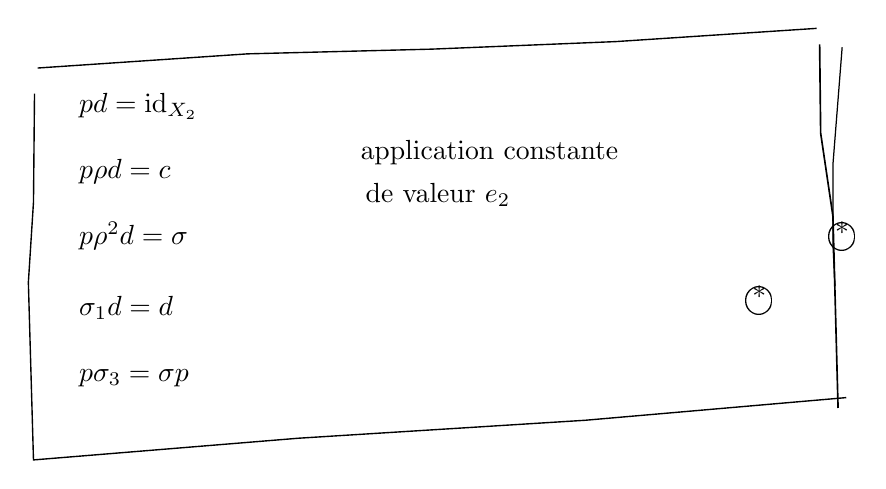
\begin{tikzpicture}[x=.013cm,y=.012cm,every node/.style={inner sep=0pt}]
\node[anchor=base west] at (65,-95) {$pd=\mathrm{id}_{X_2}$};
\node[anchor=base west] at (65,-165) {$p\rho d=c$};
\node[anchor=base west] at (340,-145) {application constante};
\node[anchor=base west] at (345,-190) {de valeur $e_2$};
\node[anchor=base west] at (65,-235) {$p\rho^2d=\sigma$};
\node[anchor=base west] at (65,-310) {$\sigma_1d=d$};
\node[anchor=base west] at (65,-380) {$p\sigma_3=\sigma p$};
\node[anchor=center] at (730,-294) {\textcircled{*}};
\node[anchor=center] at (811,-226) {\unsure{\textcircled{*}}};
\draw[line width=.5pt] (25,-48) -- (230,-33) -- (410,-28) -- (590,-20) -- (786,-6);
\draw[line width=.5pt] (22,-75) -- (21,-190) -- (16,-275) -- (21,-463) -- (280,-440) -- (560,-421) -- (815,-397);
\draw[line width=.6pt] (789,-23) -- (790,-117) -- (802,-205) -- (807,-408);
\draw[line width=.45pt] (811,-26) -- (802,-150) -- (802,-235) -- (804,-279);
\end{tikzpicture}}

\[
\unsure{\mathcal G_3|\mathfrak S_3}
=\deleted{\unsure{\{1,\rho,\rho^2\}}}\{1,\sigma_1\}\cdot\{1,\rho,\rho^2\}
=\underbrace{\{1,\rho,\rho^2\}}_{\substack{\unsure{\rotatebox{90}{$\in$}}\\g}}\cdot\underbrace{\{1,\sigma_1\}}_{\substack{\rotatebox{90}{$\in$}\\h}}
\]
\[
d(X_2)\subset X_3\qquad(g\circ h)\circ d=g\circ d
\]
\[
\begin{gathered}
[\rho^i d(\unsure{\zeta|\xi}\deleted{\unsure{'}})=\rho^{i'}d(\unsure{\zeta'|\xi'})]
\ \substack{\overset{?}{\Longrightarrow}\\[-2pt]\Longleftarrow}\
[i\equiv i'\ (3),\ \unsure{\zeta|\xi}=\unsure{\zeta'|\xi'}]\\
\Updownarrow\\
[d(\unsure{\zeta'|\xi'})=\rho^{i\deleted{\unsure{'}}-i'}d(\unsure{\zeta|\xi}\deleted{\unsure{'}})]
\end{gathered}
\]
\margin{\inserted{ou $[\unsure{\zeta|\xi}=\unsure{\zeta'|\xi'}=e_2]$}}

\[
d(\unsure{\zeta'|\xi'})=\rho^j d(\unsure{\zeta|\xi}\deleted{\unsure{'}})
\left\{\begin{aligned}
&\text{si }j=0\quad\text{on a}\quad\unsure{\zeta'|\xi'}=\unsure{\zeta|\xi}\quad\text{cqfd}\\
&\text{si }j=1\quad\text{on a}\quad\unsure{\zeta'|\xi'}=p\rho d(\unsure{\zeta|\xi})=e_2\\
&\text{donc}\quad\underset{\substack{\Vert\\\inserted{d(\unsure{\zeta'|\xi'})=d(e_2)}}}{e_3}=\rho d(\unsure{\zeta|\xi})\\
&\text{donc}\quad d(\unsure{\zeta|\xi})=e_3\quad\text{donc}\\
&\deleted{\text{donc}\quad d(\unsure{\zeta|\xi})=e_3}\\
&\unsure{\zeta|\xi}=pd(\unsure{\zeta|\xi})=pe_3=e_2\\
&\text{donc}\quad\unsure{\zeta|\xi}\deleted{\unsure{'}}=\unsure{\zeta'|\xi'}=e_2\\
&\text{si }j=2,\quad\unsure{\zeta'|\xi'}=p\rho^2d(\unsure{\zeta|\xi})=\sigma\unsure{\zeta|\xi}
\end{aligned}\right.
\]
\margin{$d\sigma(\unsure{\zeta|\xi})=\rho^2d(\unsure{\zeta|\xi})\qquad d(\unsure{\zeta|\xi})=\rho d\sigma(\unsure{\zeta|\xi})$
\[
\unsure{\zeta|\xi}=p\rho d\sigma(\unsure{\zeta|\xi}\unsure{]|)}=e_2,\quad\unsure{\zeta'|\xi'}=e_2
\]}

\margin{21}
